\documentclass[a4paper,12pt,titlepage]{article}
\usepackage{verbatim}
\newcommand{\HRule}{\rule{\linewidth}{0.5mm}}
\usepackage{float}
\usepackage{graphicx}
\usepackage[utf8]{inputenc}
\usepackage{hyperref}
\usepackage{minitoc}
\usepackage{minted}

\DeclareGraphicsExtensions{.PNG,.png,.jpg,.JPG}
\graphicspath{{./Images/}}
%\end{comment}

\begin{document}




%\newcommand{\HRule}{\rule{\linewidth}{0.5mm}}
\begin{titlepage}
\begin{center}

\includegraphics[width = 0.3\textwidth]{US_newLogo.png}~\\[1cm]
\textsc{\LARGE Unsolvable Solutions}\\
Client: Francois Mouton at the CSIR DSSR\\[1.5cm]
\textsc{\Large  Architectural Requirements}\\[0.5cm]

 \HRule\\[0.4cm]
{ \huge \bfseries  Eavesdrop \\[0.4cm] }

 \HRule\\ 



Github link:  \url{https://github.com/Unsolvable-Solutions/Project-EPIC} \\[1.2cm]

\noindent
\begin{minipage}[t]{0.4\textwidth}

	\begin{flushleft} \large
	\emph{Members:}\\
		Edwin Fullard  \\
		Jaco Bezuidenhoudt \\
		Jandre Coetzee\\
		Maret Stoffberg\\
		Ryno Pierce\\
	\end{flushleft}
\end{minipage}%
\begin{minipage}[t]{0.4\textwidth}
\begin{flushright} \large
	\emph{Student Number:} \\
		12048675 \\
		11013878 \\
		 10693077 \\
		 11071762 \\
		 12003922\\
	\end{flushright}
\end{minipage}

\vfill


% Bottom of the page




\end{center}
\end{titlepage}


\tableofcontents



\newpage
\section{System Overview}
The Malware is developed as a proof of concept for the Eavesdropping Protection in Conclave (EPIC) product. 
The Malware has the ability to eavesdrop on unsuspecting victims via their own Android device.

\section{System Configuration}
The Malware consistes of two parts: the application and the server.

The application is installed on your Android device and the server. A request to start recording is send from the server to the application to start recording by the user. The user then stops the recording and it is stored on the server.

\section{Installation}
%%TODO: meer prentjies by die intallasie deel, net soos screen shots of iets
%TODO voeg link in
%wat van nou met die browser-ding?

\subsection{Android Malware Application}
\begin{enumerate}
\item Copy the file named \textit{EPICMalware.apk} over to your device. You can download the file from \url{https://github.com/Unsolvable-Solutions/Project-EPIC/tree/master/EPICMalware/MalwareApp/Eavesdrop}.
\item Locate the file on your device and tap on the file.
\item A list of permissions will pop-up that the application needs in order to function. Click on the \textit{install} option.
\item The application is now ready to use.
\end{enumerate}

\subsection{Java Malware Server}
\begin{enumerate}
\item Make sure a minimum version of Java 7 is running on your system.
\item Download(or clone) the source files from \url{https://github.com/Unsolvable-Solutions/Project-EPIC/tree/master/EPICMalware/MalwareServer}
\item In your command line
\begin{itemize}
\item Redirect to the folder that you have just downloaded.
\item Run
\begin{minted}{python}
java -jar EPICMalwareServer.jar
\end{minted}

\end{itemize}
\item Follow the on-screen instructions.
\end{enumerate}


\section{Getting Started}


\subsection{Java Malware Server}
\begin{enumerate}
\item To use the EPICMalware application you first need to start the malware server.
Please refer to the installation of the EPICMalwareServer to start the server.
\item There are two options for using the malware server, the server can control the recording or the Android application can be used to control the recording. 
\begin{figure}[H]
\center
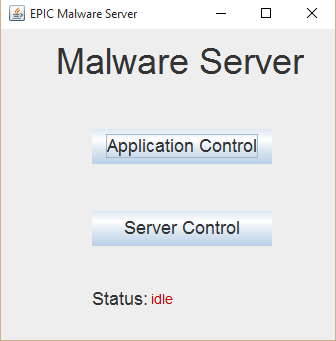
\includegraphics[height=6cm]{MalwareScreenshots/AppStart}
\caption{Malware Server main screen}
\label{fig:my_label5}
\end{figure}
\end{enumerate}

\subsection{Android Malware Application}
\begin{enumerate} 
\item Navigate to to application shortcut named \textit{Eavesdrop} on your phone and open it.
\item If application control was selected on the server the \textit{Start Recording} and \textit{Stop Recording} buttons can be used to interact with the server.
\end{enumerate}
\begin{figure}[H]
\center
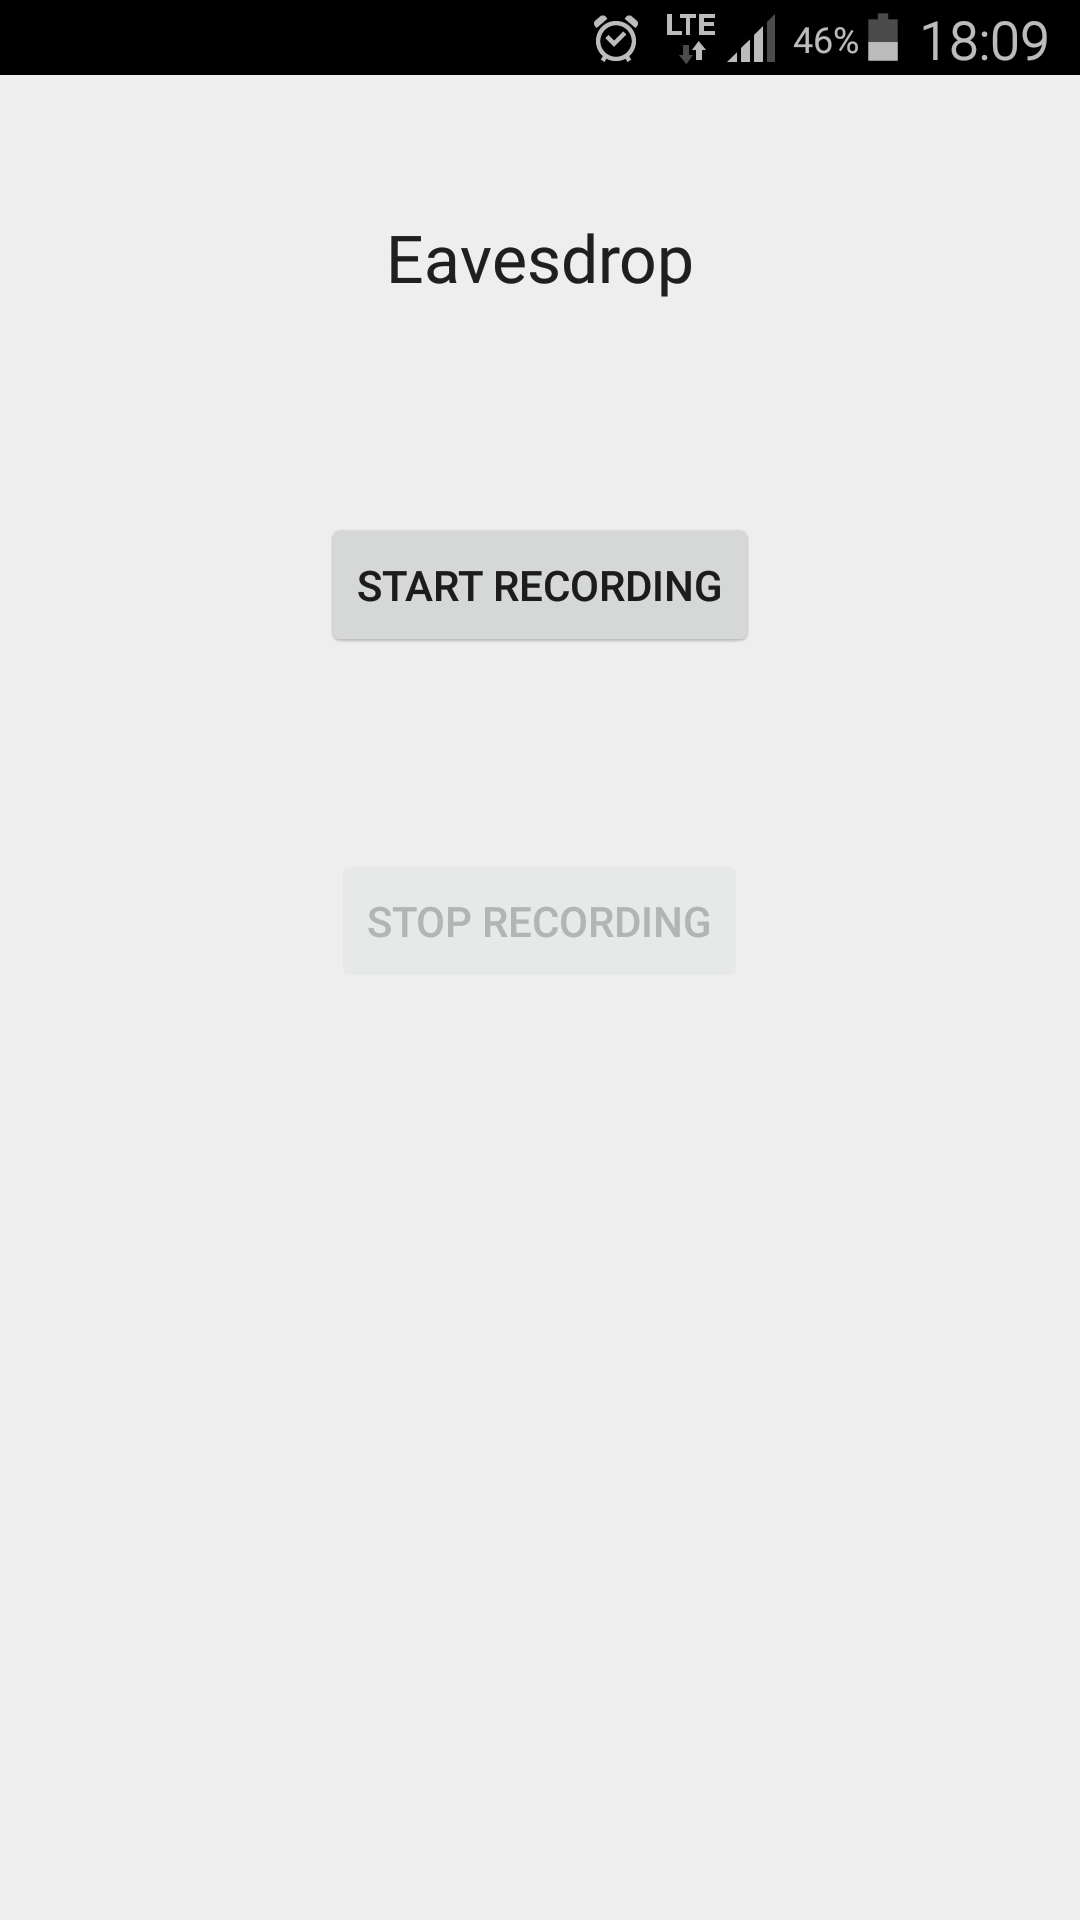
\includegraphics[height=8cm]{MalwareScreenshots/StartRecording}
\caption{Android Malware Application main screen}
\label{fig:my_label6}
\end{figure}




\section{Using The System}

\subsection{Java Malware Server}
\begin{enumerate}
\item{If application control is selected the server waits for an incoming connection and starts recording. Using this option the android application is manually controlled. When local recording and streaming needs to be stopped select yes from the stop recording, dialog this will terminate and save the recording.
\begin{figure}[H]
\center
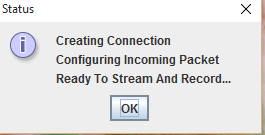
\includegraphics[width=5cm,height=3cm]{MalwareScreenshots/infoStatus}
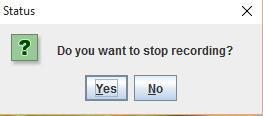
\includegraphics[width=5cm,height=3cm]{MalwareScreenshots/stopRec}
\caption{Malware Server options}
\label{fig:my_label7}
\end{figure}}
\item{If server control is selected the server will wait for incoming requests to connect to the server and add them to a list. 
\begin{figure}[H]
\center
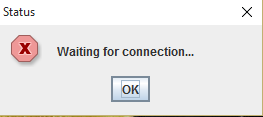
\includegraphics[width=8cm]{MalwareScreenshots/waiting}
\caption{Malware Server server control option selected}
\label{fig:my_label8}
\end{figure}
\item The user will be able to select a device from the list to eavesdrop on.
\begin{figure}[H]
\center
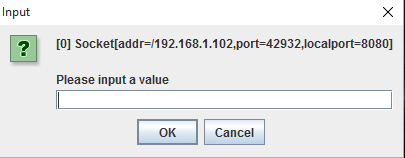
\includegraphics[width=8cm]{MalwareScreenshots/select}
\caption{Malware Server device list}
\label{fig:my_label9}
\end{figure}
\item When a device is selected from the list the server will start to record the incoming stream. 
\item When the you want to stop the recording select \textit{Yes} on the stop recording dialog and the server will terminate and save a local recoding of the stream.
\begin{figure}[H]
\center
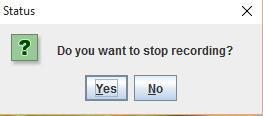
\includegraphics[width=5cm]{MalwareScreenshots/stopRec}
\caption{Malware Server recording from device}
\label{fig:my_label10}
\end{figure}}
\end{enumerate}

\subsection{Android Malware Application}
\begin{enumerate}
\item The android application can only be manually controlled when application control is selected on the Malware server.
\item After the \textit{Start Recording} button is pressed, the audio stream will be sent to the server. The \textit{Start Recording} button is now greyed out.
\begin{figure}[H]
\center
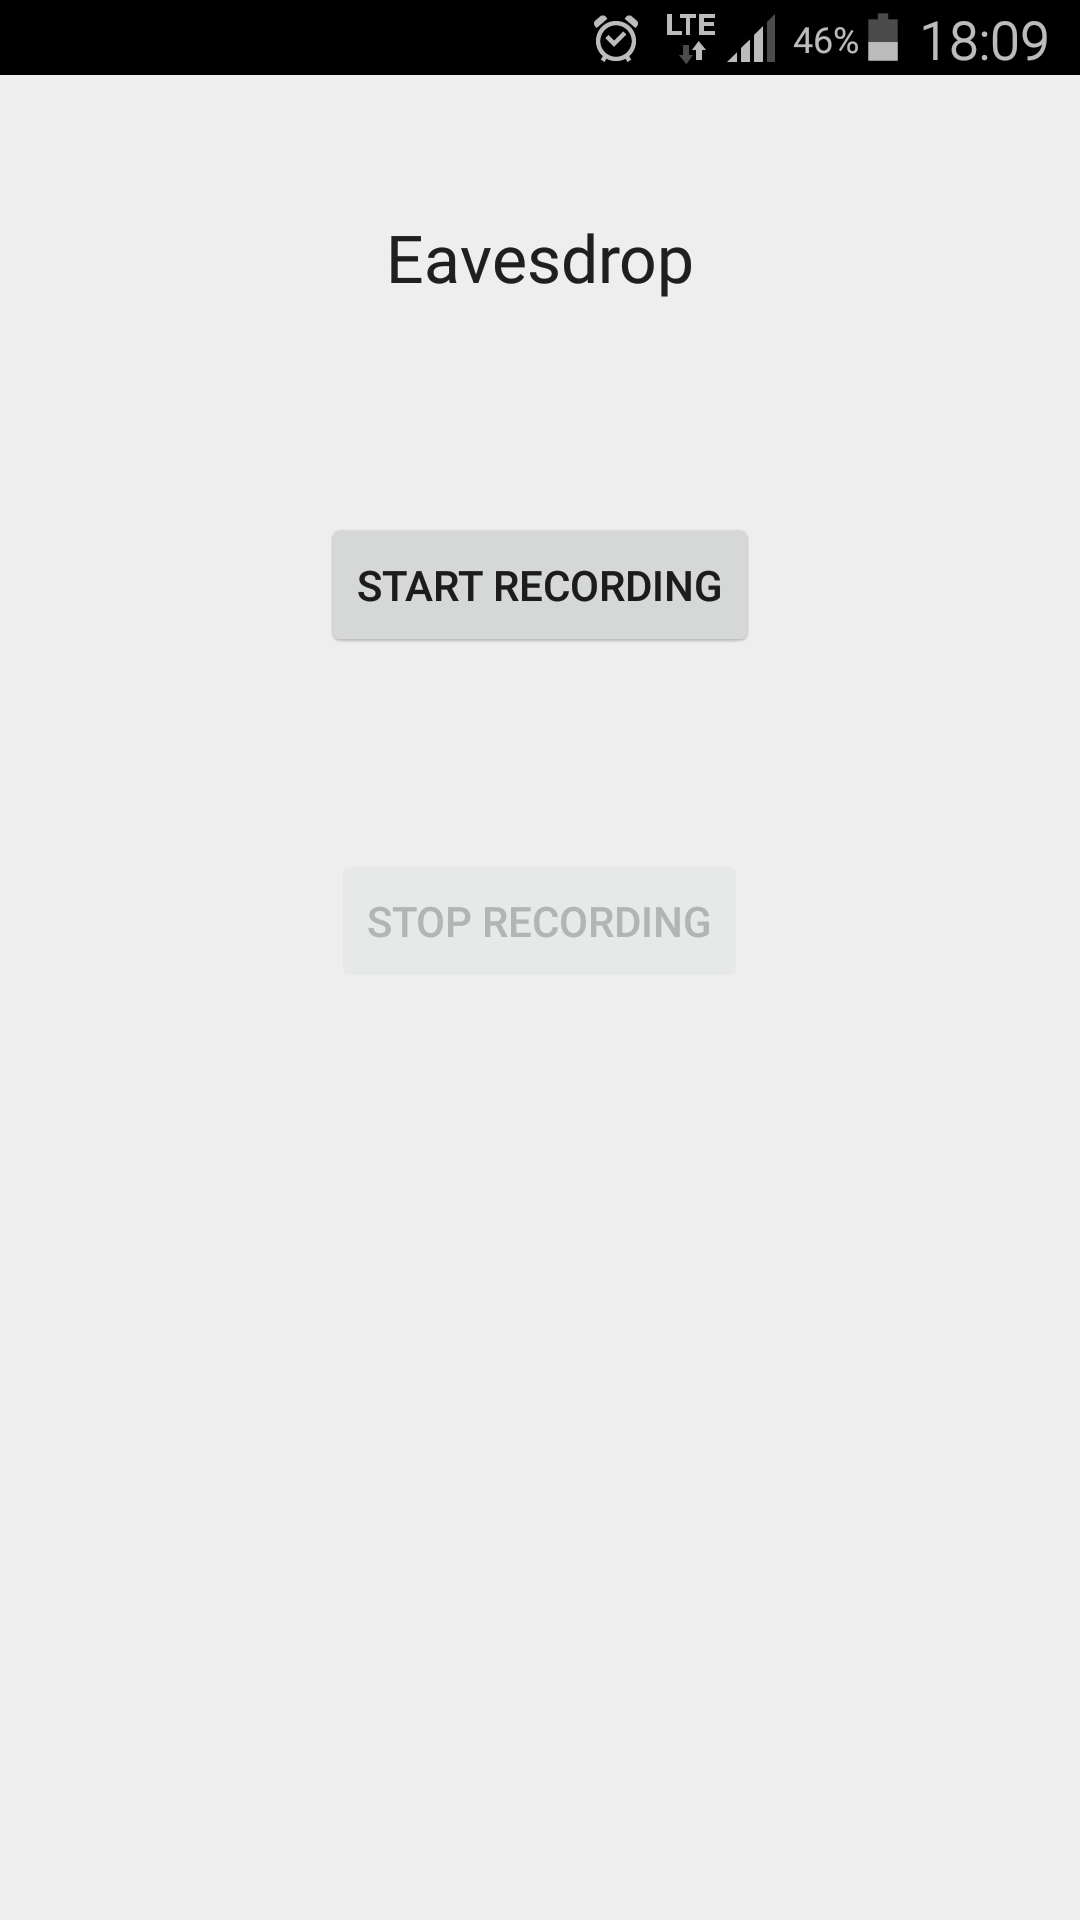
\includegraphics[ height=8cm]{MalwareScreenshots/StartRecording}
\caption{Android malware application start recording}
\label{fig:my_label11}
\end{figure}
\item After the \textit{Stop Recording} button is pressed, the application stops to send a audio stream to the server. The user must also stop the server to save a copy of the stream on the device running the server.
\begin{figure}[H]
\center
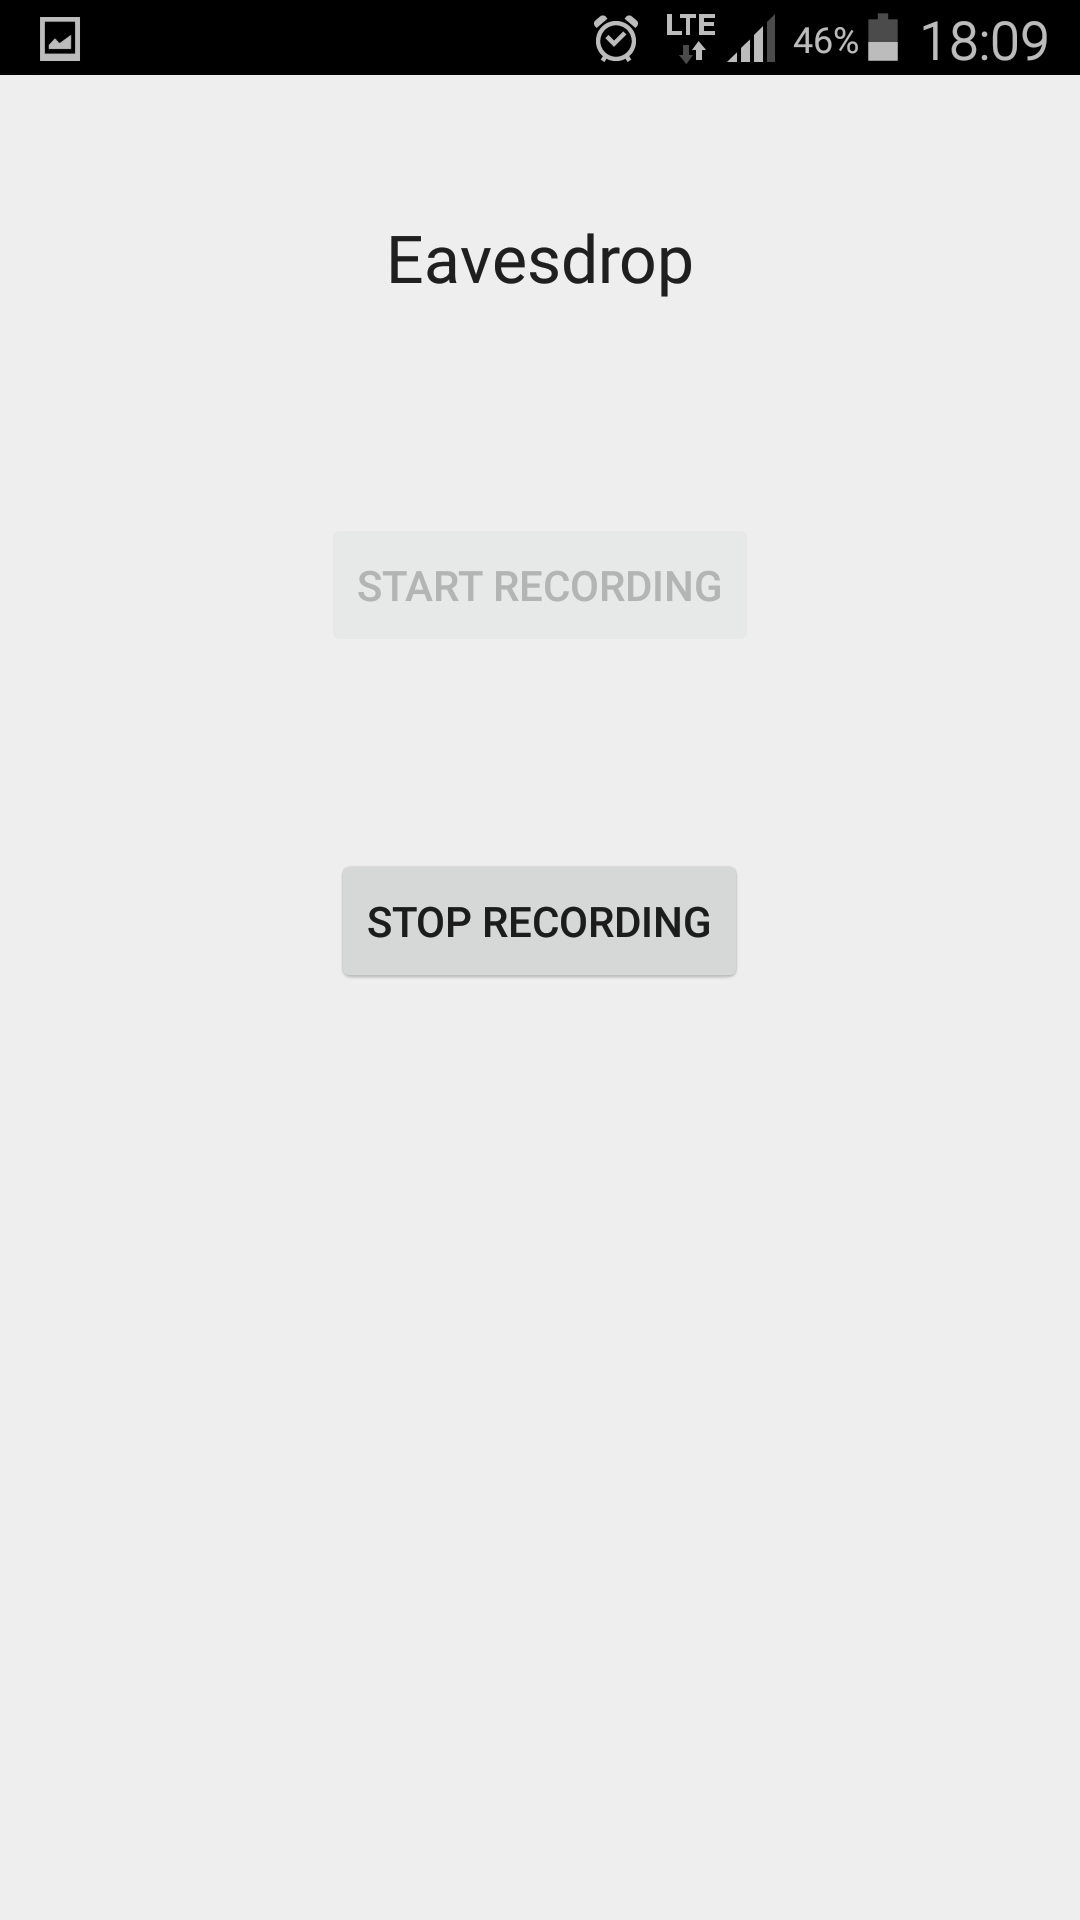
\includegraphics[ height=8cm]{MalwareScreenshots/StopRecording}
\caption{Android malware application stop recording}
\label{fig:my_label12}
\end{figure}
\end{enumerate}


\section{Troubleshooting}
\subsection{Java Malware Server}
\begin{itemize}
\item If the server cannot stream the audio or no devices are detected open ports 4545 and 8080 on your firewall. These ports are used for communication between the application and the server.
\end{itemize}
\subsection{Android Malware Application}
\begin{itemize}
\item If any problems occur within the application just restart the application.
\end{itemize}




\end{document}
